\section{Simulation Analysis and Comparison with Theoretical Values}
\label{sec:simulation}

\subsection{Frequency Analysis}
\subsubsection{Magnitude Response}

Figure~\ref{fig:gain} shows the frequency magnitude response of the circuit, for the voltage gain, which is expressed in dB. Comparing to the theoretical graphic, which is on the right, we notice that the curves are very similar. We only notice the differences by taking a closer look to both curves, and see that the maximum voltage gain is not the same for the theoretical and simulated results. Both results approach very well the reference value, 40dB, and the differences between these two results might rely on the fact that NGSpice uses a real OPAMP model.

\begin{figure}[H]
\centering
\begin{subfigure}{.5\textwidth}
    \centering
    \vspace{2.8 cm}
    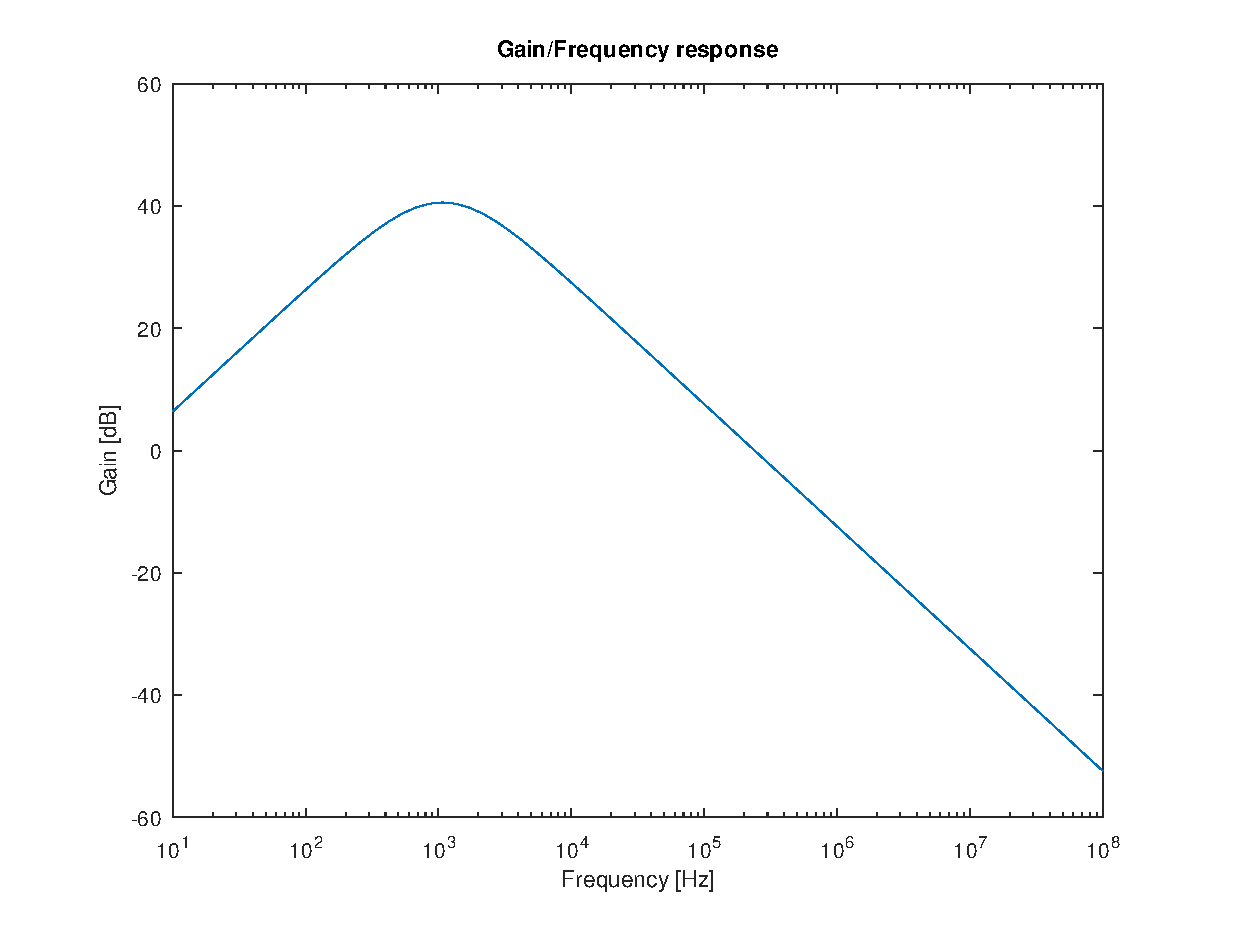
\includegraphics[scale=0.4]{gain_response.eps}
    \caption{Theoretical Phase Response}
\end{subfigure}%
\begin{subfigure}{.5\textwidth}
    \centering
    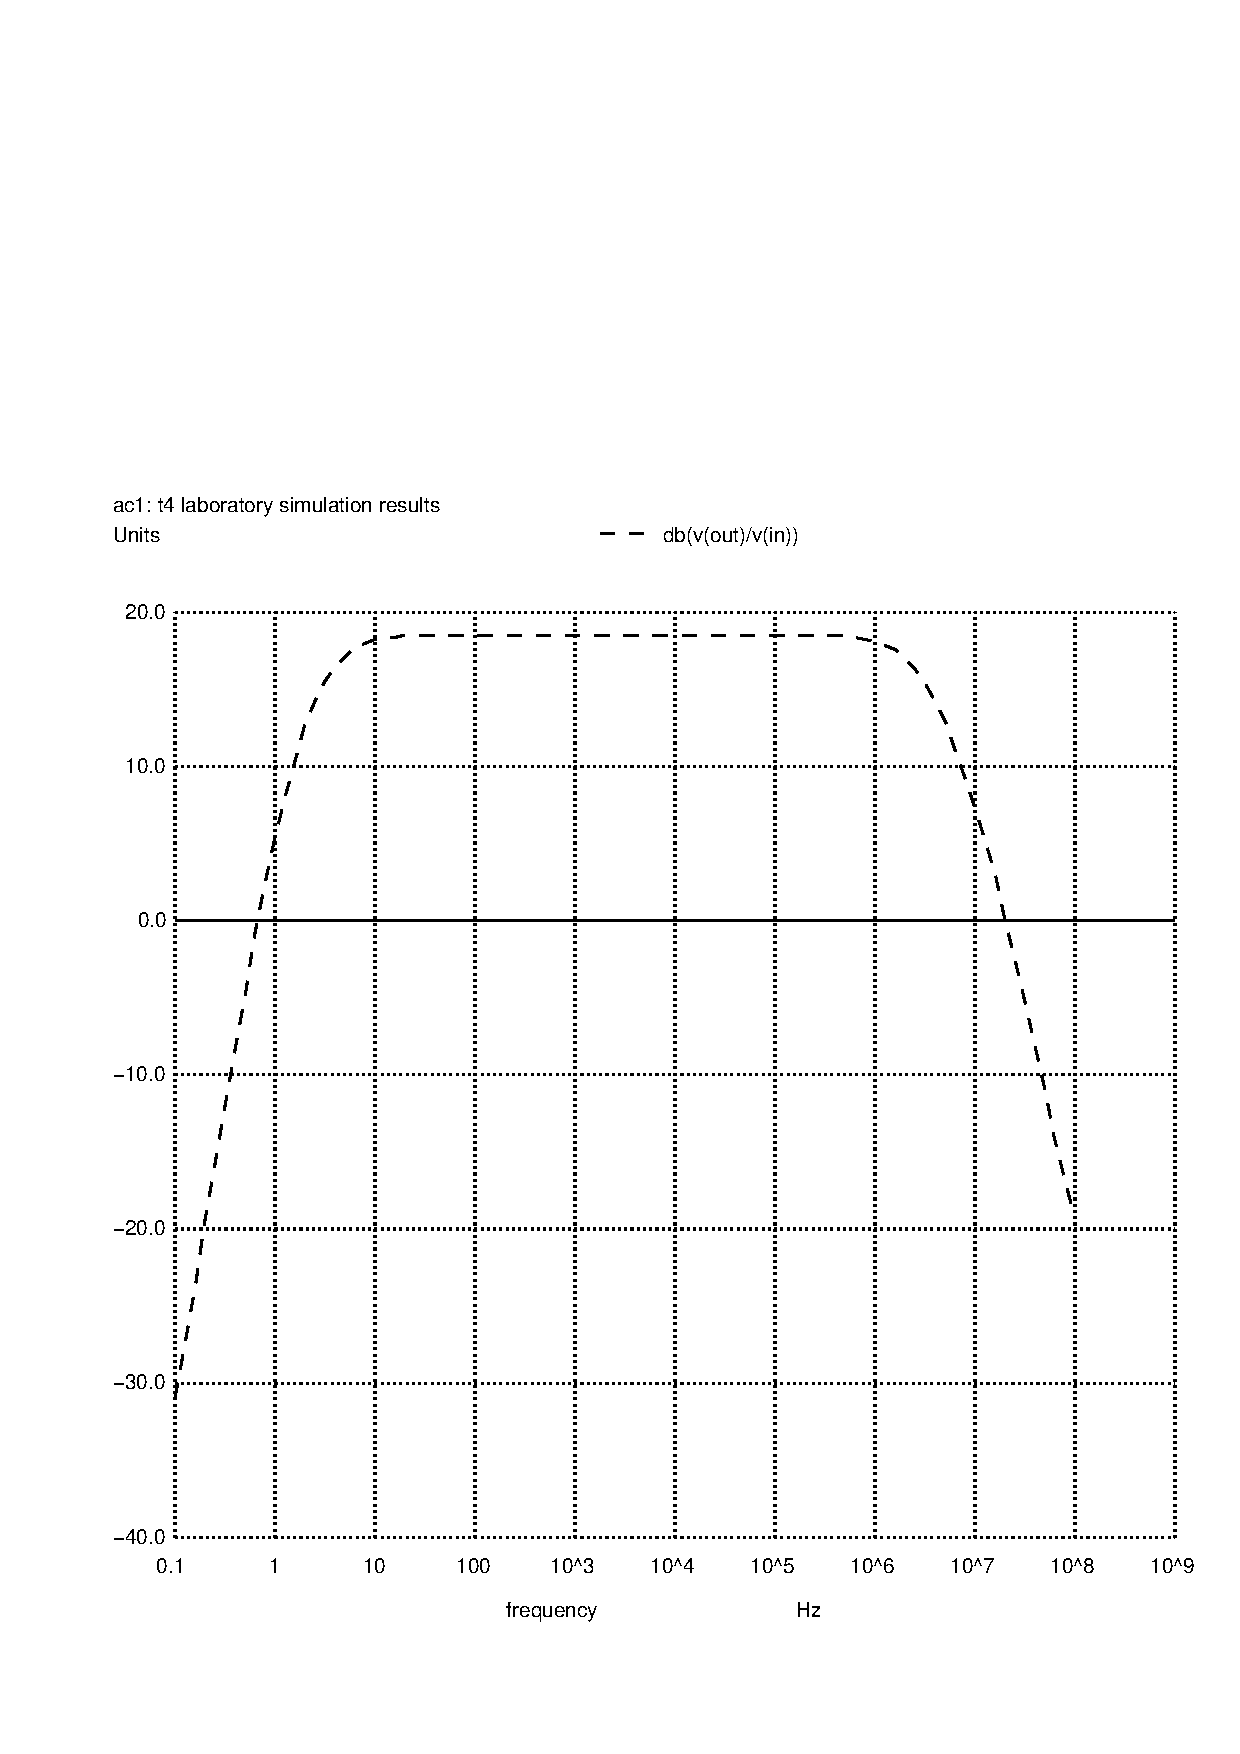
\includegraphics[scale=0.33]{gain.pdf}
    \caption{Simulation Phase Response}
\end{subfigure}
\caption{Gain Response}
\label{fig:gain}
\end{figure}



\subsubsection{Phase Response}


Figure~\ref{fig:phase} shows the frequency phase response of the circuit, for the voltage gain, which is expressed in degrees. Comparing to the theoretical graphic, which is on the right, we might consider that the curves are very different, since we see a sudden jump of phase, in the simulated graphic. However, if we take a closer look, we notice that the simulated graphic shows a jump of +180 degrees in the phase in order to fit the scale. If we ignore that necessary jump, we conclude that the theoretical curve only has 2 poles, while the simulated one has 4. That can be explained by the fact that NGSPice simulates a real OPAMP model, while Octave performs a theoretical analysis of the circuit, with an idealized OPAMP model.


\begin{figure}[H]
\centering
\begin{subfigure}{.5\textwidth}
    \centering
    \vspace{2.8 cm}
    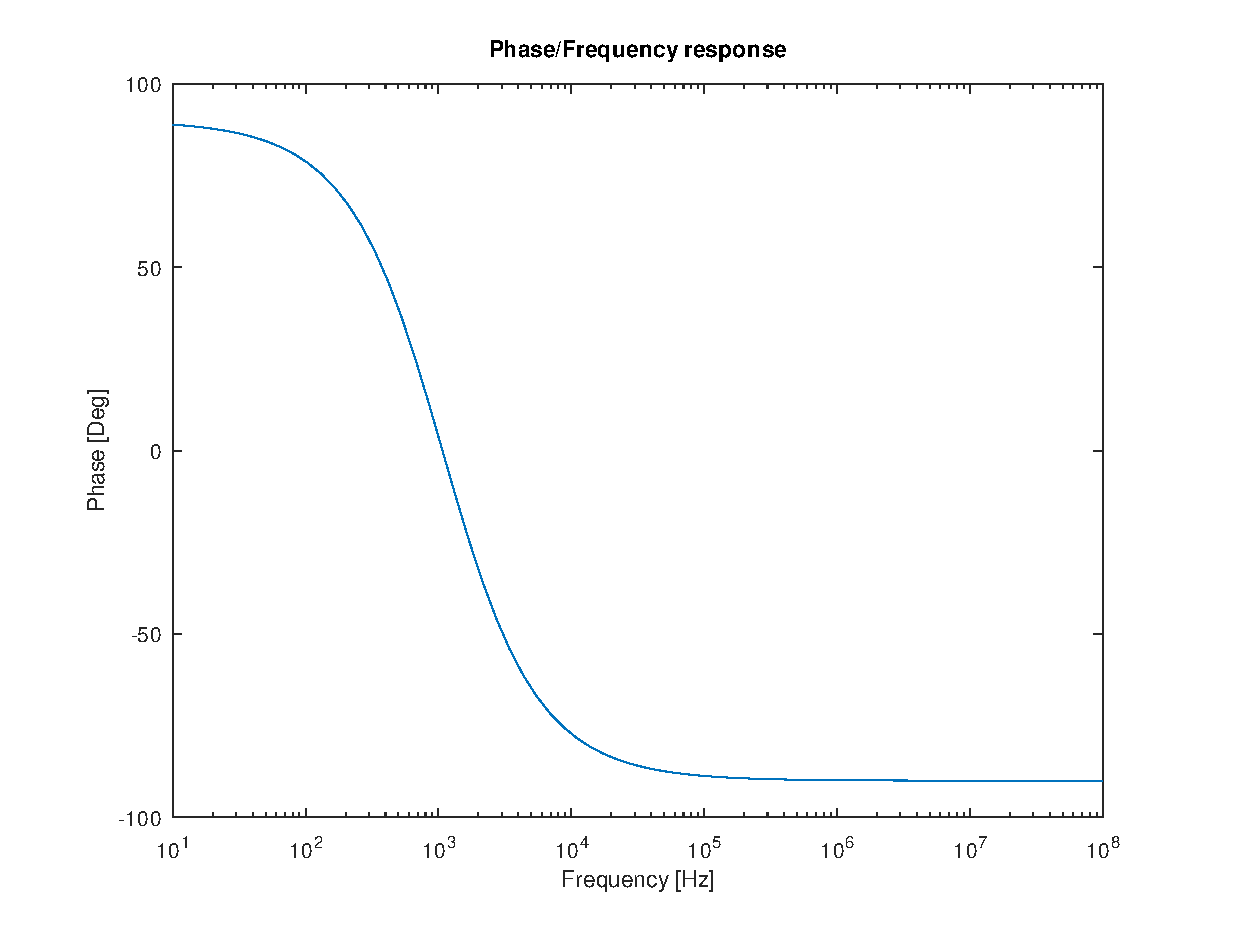
\includegraphics[scale=0.4]{phase_response.eps}
    \caption{Theoretical Phase Response}
\end{subfigure}%
\begin{subfigure}{.5\textwidth}
    \centering
    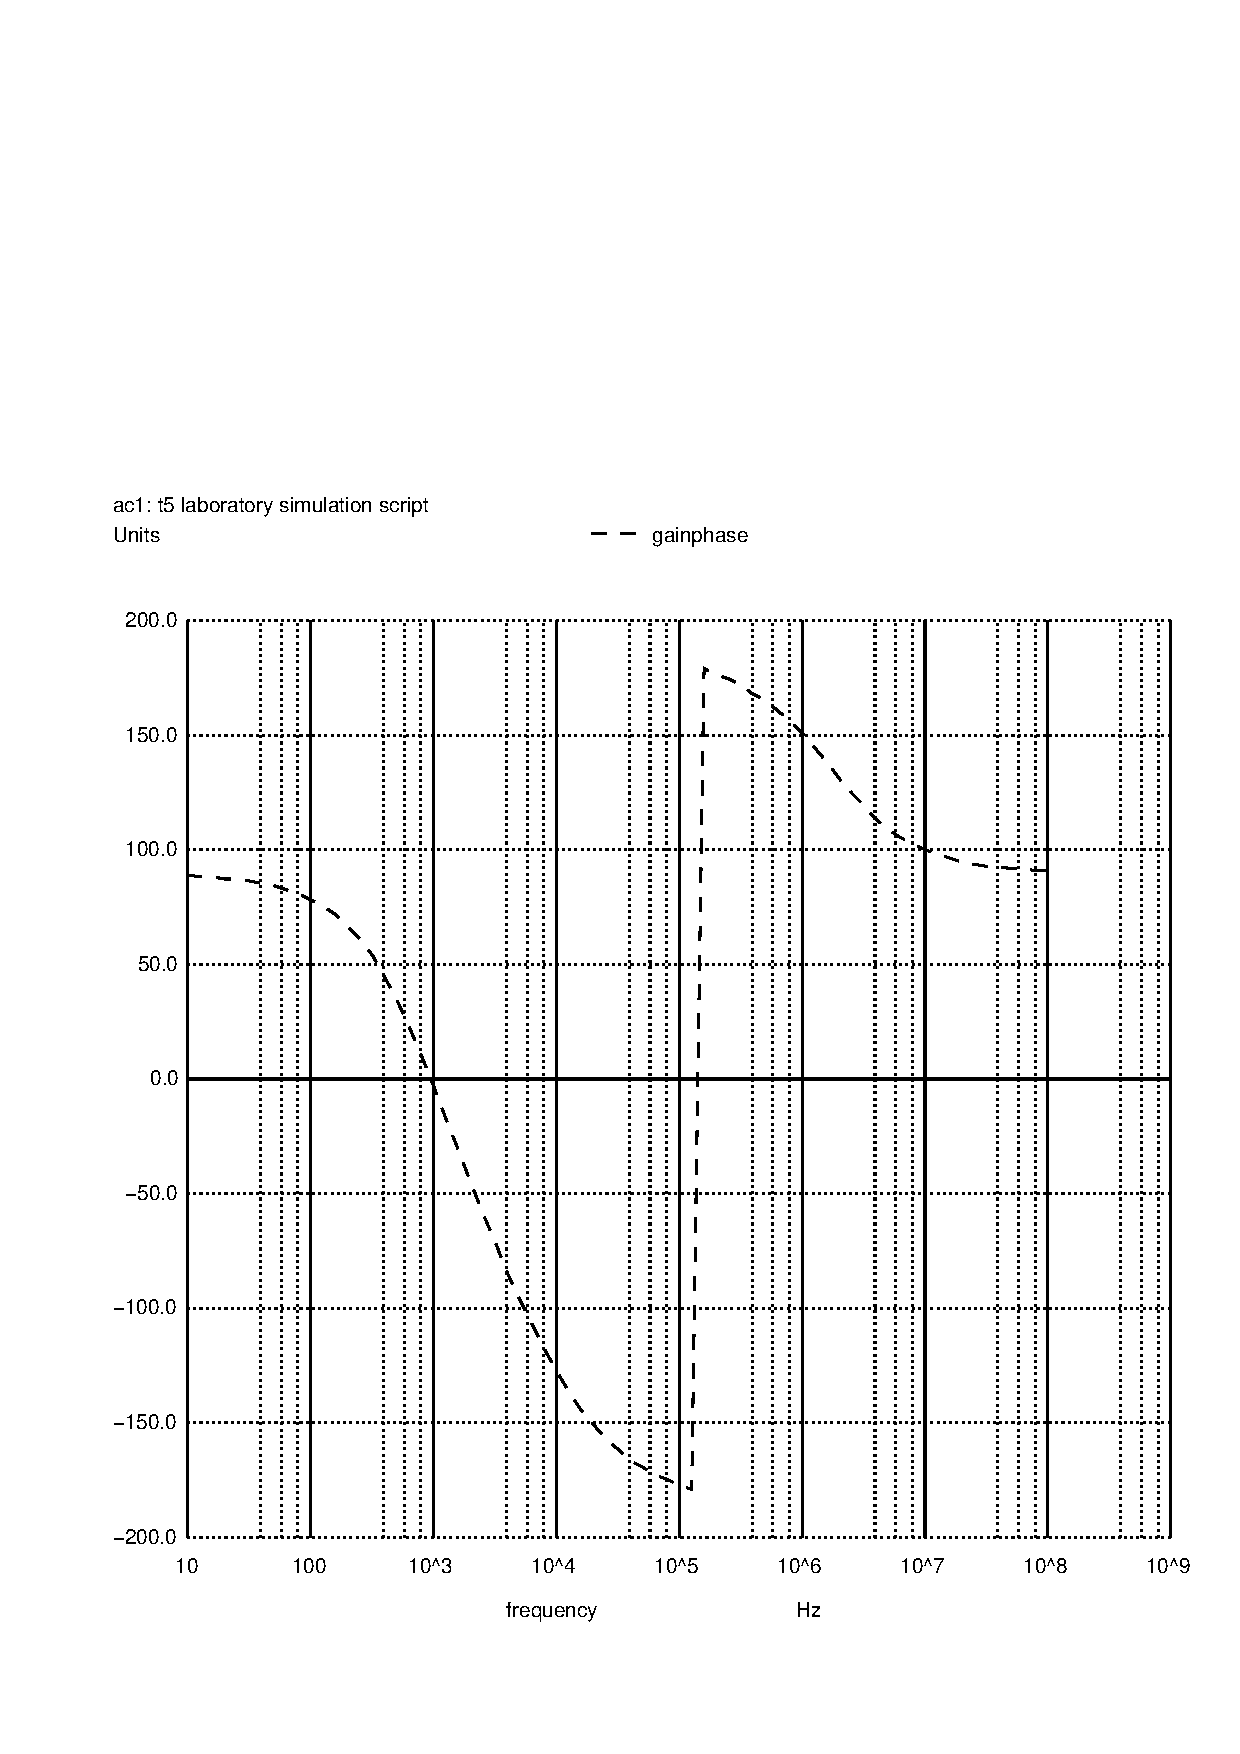
\includegraphics[scale=0.33]{phase.pdf}
    \caption{Simulation Phase Response}
\end{subfigure}
\caption{Phase Response}
\label{fig:phase}
\end{figure}



\subsection{Simulation Results}

Table~\ref{tab1:impedance} shows the simulated results, using NGSPICE, for the input and output impedances, at the central frequency. Remind that the values on the right are the theoretical ones obtained by Octave, which are reproduced in this section to help compare them to the simulated resuls. Comparing both the values, we conclude that the results are very close, some differences resulting on the fact that, on NGSpice, we used an aproximate value of the central frequency to calculate the impedances and because in this simulating tool, it considers the components real (the OPAMP, most importantly).


\begin{table}[H]
  \begin{tabular}{|l|r|}
    \hline    
    {\bf Name} & {\bf Ohm} \\ \hline
    zin & 1.161859e+03\\ \hline

  \end{tabular}
  \begin{tabular}{|l|c|}
    \hline
    {\bf Name} & {\bf Value} \\ \hline
    $Z_{in}$ & 9.090909e+02 + j-6.741999e+02 Ohm \\ \hline
$Z_{out}$ & 6.451613e+02 + j-4.784644e+02Ohm \\ \hline
$|Z_{in}|$ & 1.131809e+03 Ohm \\ \hline
$|Z_{out}|$ & 8.032193e+02 Ohm \\ \hline

  \end{tabular}
  \begin{tabular}{|l|c|}
    \hline
    {\bf Name} & {\bf Ohm} \\ \hline
    zout & 8.251525e+02\\ \hline

  \end{tabular}
    \caption{Comparison of Input and Output Impendances (Left - Simulation Values, Right - Theoretical Values)}
    \label{tab1:impedance}
\end{table}

Finally, Table~\ref{tab:merit} shows the values obtained for the gain and central frequency of the circuit under analysis. The table shows also the merit result and the values used for the calculation of the merit figure, which are the cost, the central frequency deviation (which should be ideally 1kHz) and the linearly voltage gain deviation (which should be ideally 100).

\begin{table}[H]
    \begin{tabular}{|l|c|}
    \hline
    {\bf Name} & {\bf Value} \\ \hline
    $AV_{HP}$ & -1.903317e+00 dB \\ \hline
$AV_{OPAMP}$ & 4.440216e+01 dB \\ \hline
$AV_{LP}$ & -1.903317e+00 dB \\ \hline
$AV$ & 4.059553e+01 dB \\ \hline

  \end{tabular}
  \begin{tabular}{|l|r|}
    \hline    
    {\bf Name} & {\bf Value} \\ \hline
    Gain(dB)&37.0419\\ \hline
Gain& 71.1371\\ \hline
Central Frequency(Hz)& 1051.2\\ \hline
Gain deviation&28.8629\\ \hline
Central frequency deviation(Hz)&51.2041\\ \hline
Cost(MU)& 13446.7\\ \hline
Merit & 9.28821E-07\\ \hline

  \end{tabular}
  \begin{tabular}{|l|c|}
    \hline
    {\bf Name} & {\bf Value} \\ \hline
    $w_{L}$ & 5.000000e+03 rad/s \\ \hline
$w_{H}$ & 9.090909e+03 rad/s \\ \hline
$w_{O}$ & 6.741999e+03 rad/s \\ \hline
$f_{O}$ & 1.073022e+03 Hz \\ \hline

  \end{tabular}
    \caption{Comparison of Gain (Left - Theoretical Values, Right - Simulation Values)}
    \label{tab:merit}
\end{table}

Comparing to the theoretical results, we can see that both results aproach closely the reference values. However, we can notice some slight differences on the gain and the central frequency results, which can be explained by the fact that NGSPice simulates a real OPAMP model, while Octave performs a theoretical analysis of the circuit.

Lastly, as one can notice, we achieved a very low merit value. However, if we analyse the restrictions imposed on the uses of certain components and the results for the gain and the central frequency, which are quite close to the reference values, we conclude that, despite the low merit value, we achieved a very efficient circuit whose quality would degrade significantly if we changed randomly the values of the components to achieve the highest merit figure possibly. 
